\chapter{Production de l'énergie électrique}
\section{Généralités}
\subsection{Définition d'un cycle combiné}
Un cycle combiné est l'association de  deux cycles thermodynamiques. \\
Une centrale à cycle combiné\footnote{Généralement appelée CCGT (Combined Cycle Gaz Turbine) ou TGV (Turbine Gaz-Vapeur)} est une centrale thermique qui relie deux types de turbines : turbine à gaz et turbine à vapeur.

Le principe de fonctionnement d'un cycle combiné repose sur l'alimentation d'une turbine par les échappements d'une autre. De cette façon, on peut extraire plus d'énergie pour une même consommation en combustible.\\ Du coup, l'efficacité du système augmente.     %a revoir
\begin{figure}[h]
\centering
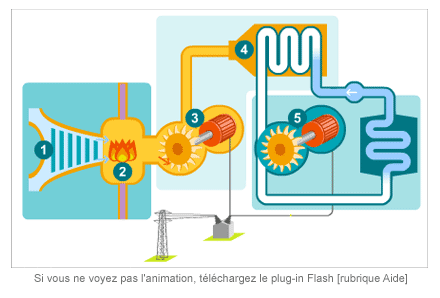
\includegraphics[scale=0.5]{./Figures/principe_cycle_combine.png}
\caption{Principe de fonctionnement du cycle combiné}
\end{figure}

Dans une centrale à cycle combiné, les gaz issus de la combustion à haute température (pouvant atteindre les 1.500 \textcelsius), actionnent une turbine à gaz. En sortie, les gaz sont encore suffisamment chauds (entre 400 \textcelsius\  et 650 \textcelsius\ environ) pour générer de la vapeur dans une chaudière au moyen d'un échangeur de chaleur. La vapeur ainsi produite entraîne une turbine à vapeur. Il est enfin nécessaire de disposer d'une source froide pour évacuer la chaleur nécessairement produite par le cycle. 

\begin{comment}
Chacune de ces turbines entraîne une génératrice qui produit de l'électricité (configuration "multi-arbres" ou "multi-shaft") ou les deux types de turbines sont couplées à la même génératrice (configuration "single-shaft").

De nombreuses possibilités de turbines sont alors envisageables. On peut par exemple avoir : 

\begin{itemize}
\item Une turbine à gaz, une turbine à vapeur et un alternateur sur la même ligne d'arbre
\item Une turbine à gaz avec son alternateur et une turbine à vapeur avec son alternateur
\item Deux turbines à gaz avec chacune son alternateur et une turbine à vapeur avec son alternateur
\end{itemize}

La configuration "multi-arbres" a l'avantage de permettre le démarrage et la montée en puissance rapide des turbines à gaz, la turbine à vapeur ayant généralement des temps de démarrage et de montée en puissance plus grands. La configuration "single-shaft" diminue le nombre de machines, donc l'encombrement, mais démarre plus lentement.
\end{comment}
\subsection{Fiche technique de la centrale}
La centrale de la CPC est une centrale à cycle combiné : 1 VEGA 209 E 2PAF

\begin{table}[h]
\centering
\begin{tabular}{|c|c|}
\hline
1 & Nombre de tranches identiques\\
\hline
VEGA & Vapeur et Gaz\\
\hline
2 & Nombre de TG par TV\\
\hline
9E & Type de la TG\\
\hline
2p & Cycle eau/vapeur\\
\hline
AF & Feux additionnels\\
\hline
\end{tabular}
\caption{Fiche technique de la centrale}
\label{tab:fiche_tech}

\end{table}

Elle est  principalement constituée de :

\begin{itemize}
\item Deux Turbines à gaz 115 MW (General Electric) Modèle MS9001E 
\item Une Turbine à vapeur 240 MW (ALSTOM)
\item 	Deux Chaudières de récupération (Aalborg HP-97 bar, BP-5 Bar)
\item 	Quatre Diesels de Démarrage (1.2 MW-Cummins)
\item 	Du Gaz naturel  (S.T.E.G 20-25 Bar)
\item 	Un système de contrôle commande (ALSTOM)
\item 	Du fuel de secours (Deux tanks de 10 000  \(m^3\)  Diesel)
\item 	Trois Transformateurs principaux
\item 	Deux Transformateurs de soutirages  
\item 	Une usine de traitement des eaux (IONICS 2 X 366 \(m^3\)/j eau déminéralisée)

\end{itemize} 

Ces équipements fournissent une puissance brute en pleine charge de :

\begin{tabular}{l c l}
364.4 MW &:& Sans feux additionnels (Bruleurs) \\
461,8 MW &:& Avec feux additionnels  %a verfiier

\end{tabular}


\section{Fonctionnement de la centrale}
Pour produire l'énergie électrique, la centrale de CPC adopte la configuration de deux turbines à gaz accouplées avec une turbine à vapeur.

L'air, nécessaire à la combustion, passe en un premier lieu par un système de filtration. Il est ensuite refoulé par un compresseur à 17 étages vers les 14 chambres de combustion sous une pression approchant les 10 bar. Dans ces chambres, l'air comprimé est mélangé avec le combustible (gaz ou fuel). Une fois enflammé, la réaction produit des gaz chauds. Ces derniers, guidés par les conduites de flammes, sont propulsés vers une turbine dont ils activent la rotation.
L'arbre de la turbine tourne à une vitesse angulaire approchant les 3000 tours par minute (50 Hz), lequel accouplé avec un alternateur qui génère l'énergie électrique. 
%altenateur refroidi

S'il s'agissait d'un cycle ouvert, les gaz d'échappement seraient rejetés à l'atmosphère.
Mais\footnote{Un registre inverseur (\textbf{damper}), installé entre l'échappement de chaque TG et sa HRSG (chaudière), permet aux turbines de fonctionner soit en cycle ouvert soit en cycle combiné} puisqu'il est question d'une centrale à cycle combiné, la chaleur des gaz dégagée par les deux turbines à gaz est récupérée par la chaudière de récupération associée.

L'énergie thermique du gaz est utilisée pour transformer l'eau de mer déminéralisée en vapeur sèche.
Les lignes de vapeur principales BP (Basse pression) et HP (Haute Pression) de chaque chaudière alimentent respectivement les deux ballons BP et HP.

La vapeur est envoyée sous pression vers les corps correspondants de la turbine (Corps BP, Corps HP).. Ces derniers sont  mis en mouvement et transforment l'énergie thermique en énergie mécanique. Là aussi, un alternateur transforme cette énergie en énergie électrique.

En sortie de la turbine, la vapeur est envoyée vers le condenseur dans lequel circule de l'eau froide qui permet de retransformer la vapeur en eau et le cycle recommence.

Pour plus de détails, voir Annexe \uppercase\expandafter{\romannumeral 2}.

La centrale peut fonctionner suivant trois modes: 
\begin{table}[h]

\centering
\begin{tabular}{|c|c|c|}
\hline
Cycle ouvert  & 2 TG (2 * 115 MW) &  230 MW\\
\hline
Demi-cycle  & TG (115 MW)  + TV (120 MW)  & 235 MW \\
\hline
Cycle combiné  & 2 TG (2 * 115 MW) + TV (240 MW)   & 470 MW \\
\hline
\end{tabular}
\caption{Différents types de cycles}
\end{table}



\section{Principaux compartiments de la centrale }
\subsection{Bloc Turbine à Gaz}
\begin{figure}[hbtp]
\centering
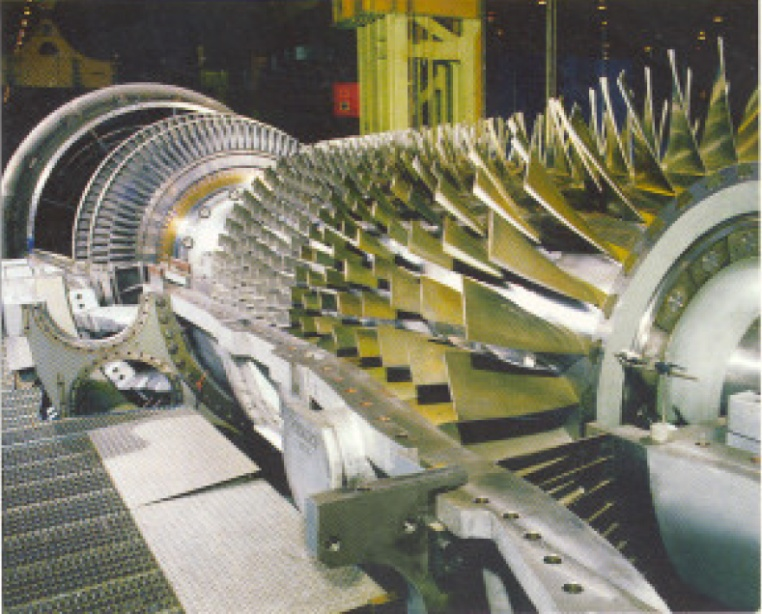
\includegraphics[scale=1]{./Figures/tg.jpg}
\caption{Turbine à Gaz MS9001E}
\end{figure}
\subsubsection{Définition d'une Turbine à Gaz }
Une turbine à gaz est une machine thermique ayant pour rôle la production d'énergie mécanique (sous forme de rotation d'arbre ) à partir d'énergie calorifique. La centrale de CPC utilise une turbine de détente des gaz chauds à 3 étages à échappement axial. Elle brûle principalement du gaz, mais peut également brûler du fuel en secours.

Le bloc Turbine à Gaz est constitué par :

\begin{itemize}
\item Un moteur auxiliaire de lancement
\item Un compresseur
\item 14 chambres de combustion
\item Une turbine
\item Un alternateur
\end{itemize}


\subsubsection{Fonctionnement}
La turbine à gaz ainsi que le compresseur, étant en position de repos, nécessitent une action extérieure pour démarrer.
C'est là ou intervient le moteur de démarrage qui met ces organes en mouvement.
Ce démarrage ne s'effectue pas de manière brusque (hâtive) et passe par différentes étapes (voir Annexe \uppercase\expandafter{\romannumeral 3}).
   

\begin{figure}[htb]
\centering
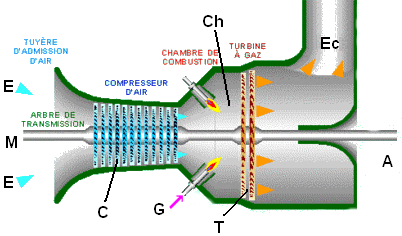
\includegraphics[scale=1]{./Figures/coupe_tg.png}
\caption{Coupe transversale d'une Turbine à Gaz.        }
Légende : \hbox{(M) Arbre} (E) Air atmosphérique     (C) Compresseur \hbox{(Ch) Chambres de combustion} (Ec) Gaz chauds  (T) Turbine (G) Bruleurs (A)\hbox{ Chaudière}.
\end{figure}

Dès que le système de démarrage de la turbine est activé, l'air ambiant est aspiré, filtré puis compressé dans les 17 étages du compresseur axial. 
 
L'air comprimé en provenance du compresseur pénètre dans l'espace annulaire à la périphérie des 14 chambres de combustion, d'où il s'introduit entre les enveloppes intermédiaires et les tubes de flamme. 

Les injecteurs introduisent le combustible dans chacune des 14 chambres de combustion où il se mélange à l'air. L'allumage s'effectue grâce à deux bougies rétractables.

Au moment où l'allumage se produit au niveau d'une des deux bougies équipant ces chambres, la combustion se propage dans les autres chambres à travers des tubes d'interconnexion qui les relient entre elles au niveau de la zone de combustion. 

Les gaz chauds issus des chambres de combustion se propagent à travers les pièces de transition emboîtées à l'extrémité arrière de chaque tube de flamme pour traverser ensuite les trois étages turbine et la faire tout en continuant leurs chemin vers le cadre d'échappement. 

Enfin, la rotation résultante de l'arbre entraîne le rotor de l'alternateur avec une vitesse de 3000 tours par minute et produit une énergie électrique de l'ordre de 115 MW. Ce dernier est réfrigéré par l'air ambiant afin d'éviter tout risques de surchauffage \cite{manuel}.

\subsection{Chaudière}
\begin{figure}[hbtp]
\centering
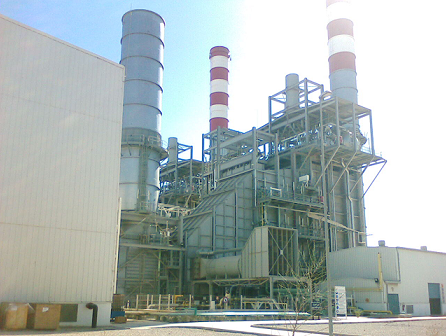
\includegraphics[scale=1]{./Figures/chaudiere.png}
\caption{Vue latérale des deux chaudières}
\end{figure}

\subsubsection{Définition}
Une chaudière ou HRSG\footnote{Heat Recovery Steam Generator} est un générateur de chaleur qui récupère la chaleur du gaz chaud \footnote{Exemple : les gaz d'échappement des deux turbines à gaz}. Elle produit de la vapeur utilisée pour alimenter une turbine à gaz.
\subsubsection{Éléments constitutifs}
Une chaudière est constituée par :

\begin{itemize}
\item Deux économiseurs (BP / HP) pour réchauffer l'eau avant de passer aux ballons BP
\item Deux évaporateurs (BP / HP) pour produire la vapeur saturée
\item Deux surchauffeurs (BP / HP) pour surchauffer la vapeur avant l'alimentation de la turbine
\item Deux ballons de chaudière (BP / HP) pour séparer la vapeur saturée de l'eau chaude

\end{itemize} 
\subsubsection{Fonctionnement}
\begin{figure}[hbtp]
\centering
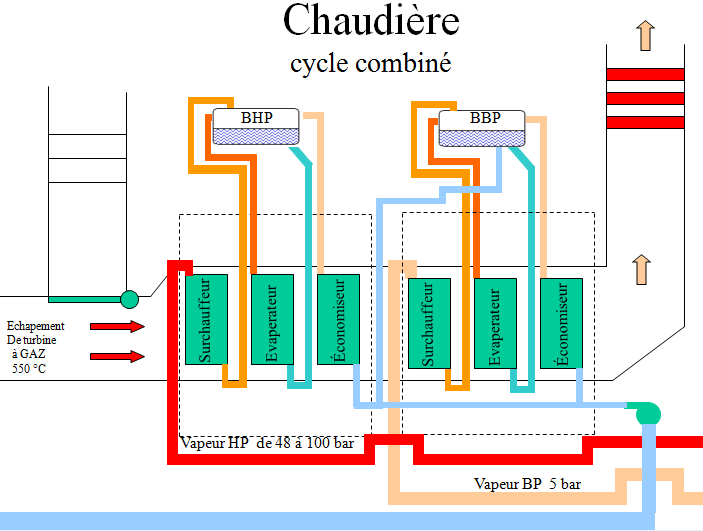
\includegraphics[scale=0.7]{./Figures/chaudiere_fonctionnement.png}
\caption{Schéma Chaudière }
\end{figure}
Le gaz d'échappement de la Turbine à Gaz de température 550 \textcelsius\ est récupéré par la chaudière. Il sert en effet à faire passer l'eau de mer traitée (voir station traitement d'eau) par différentes transformations pour obtenir une vapeur sous haute température. Cette dernière est envoyée selon sa pression (BP / HP) vers le corps correspondant de la turbine.

Dans un premier lieu, l'eau d'alimentation passe par l'économiseur BP. Son rôle est de récupérer une partie des calories restantes dans les gaz de combustion pour réchauffer l'eau avant de la passer aux ballon BP. Cette eau est ensuite transmise à l'évaporateur où est elle est pulvérisée. Le gaz produit est enfin récupéré par le surchauffeur. Il sert à élever la température de cette vapeur   afin d'en éliminer toute trace d'humidité. La vapeur sèche sous basse pression (BP) alors  est utilisée pour alimenter le corps BP de la turbine à vapeur.

Restant un  espace à exploiter dans la chaudière, l'eau passe, en deuxième lieu, par les mêmes étapes  que la partie précédente à l'exception de la présence de deux surchauffeurs. La continuité du cycle est assurée par la liaison des deux ballons\footnote{La vapeur est extraite du ballon BP pour alimenter le ballon HP}. Il est  à noter que conditions et les caractéristique de l'eau diffèrent pour obtenir à la fin de la vapeur sèche sous haute pression (HP). Cette dernière sert en effet à alimenter le corps HP de la turbine à vapeur.
\subsection{Bloc Turbine à Vapeur}
\subsubsection{Définition d'une Turbine à Vapeur}
La turbine à vapeur est une machine thermique transformant l'énergie calorifique de la vapeur d'eau en énergie mécanique de rotation. Une TV est composée de tuyères, d'ailettes, un corps basse pression (BP) et d'un corps haute pression (HP).
\begin{figure}[hbtp]
 \centering
 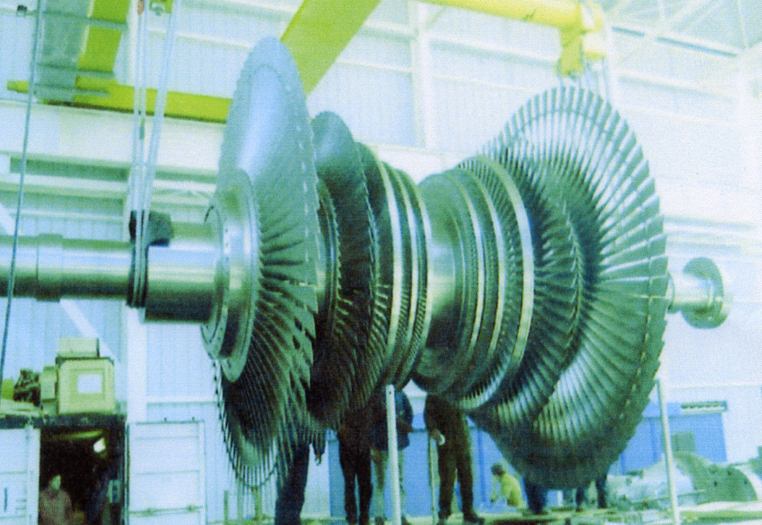
\includegraphics[scale=0.5]{./Figures/TV.png}
 \caption{Turbine à Vapeur}
 \end{figure}

\subsubsection{Fonctionnement} 
La turbine à vapeur est constituée de tuyères et d'ailettes. La vapeur s'écoule dans les tuyères dans lesquelles elle se dilate. Ainsi, sa température diminue et son énergie cinétique augmente.

La vapeur en mouvement exerce une pression contre les ailettes, entraînant la rotation de l'arbre de la turbine. 
Ce dernier, étant lié à un alternateur, tourne à 3000 tours par minute et fournit une énergie électrique de l'ordre de 120 MW sans feux additionnels (Brûleurs). Dans le cas où les deux turbines à gaz fonctionnent ensemble et avec feux additionnels, la turbine à vapeur produit 240 MW.

Contrairement aux alternateurs des turbines à gaz, l'alternateur accouplé à la turbine à vapeur est refroidi à l'hydrogène en raison de plus hautes contraintes thermiques.

Enfin, la vapeur est récupérée par le condenseur où elle regagne sa forme liquide. L'eau est en dernier temps renvoyée vers la chaudière pour alimenter les ballons BP et HP. 
\begin{figure}[hbtp]
\centering
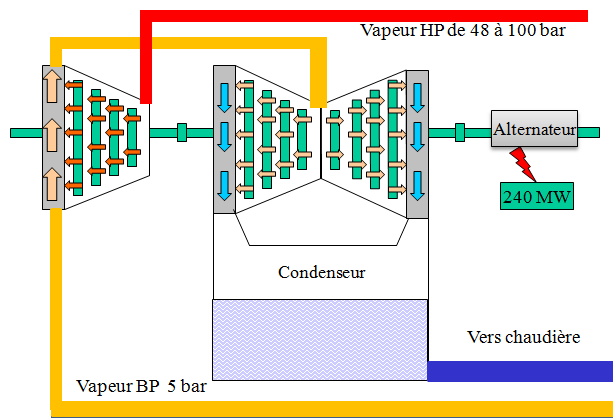
\includegraphics[scale=0.8]{./Figures/echange_tv.png}
\caption{Fonctionnement de la Turbine à Vapeur}
\end{figure}
\subsection{Condenseur}
\begin{figure}[hbtp]
\centering
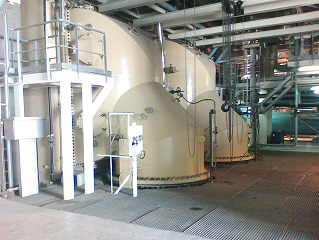
\includegraphics[scale=0.9]{./Figures/condenseur.png}
\caption{Condenseur}

\end{figure}
\subsubsection{Définition}
Le condenseur est un échangeur de chaleur dont la fonction principale est de condenser la vapeur à l'aide d'un fluide réfrigérant. La chaleur latente de la vapeur est transférée dans le fluide réfrigérant.

Dans notre cas, le fluide réfrigérant est  l'eau. 


\subsubsection{Fonctionnement}
Le condenseur sert à refroidir la vapeur issue de la turbine vapeur à l'eau CRF.

Une pompe  à vide aspire la vapeur à l'issue de la turbine.
Des centaines de tubes parcourus par l'eau de réfrigération servent à condenser la vapeur.
L'eau ainsi obtenue regagne la chaudière à travers la pompe CEX.
 
\subsection{Transformateurs}
\subsubsection{Situation}
La production de l'énergie électrique se fait en utilisant trois alternateurs :

\begin{itemize}
\item Groupe turboalternateur de la turbine à gaz A  : 15 KV
\item Groupe turboalternateur de la turbine à gaz B  : 15 KV
\item Groupe turboalternateur de la turbine à vapeur : 18 KV
\end{itemize}

   L'énergie  produite  est  évacuée  vers  le  réseau  à  travers  des  disjoncteurs (de groupes et de lignes)  à  haute tension assurant l'isolement automatique du groupe en cas de danger.
  

Cependant, les tensions récupérées sont soit insuffisants (pour les vendre à la STEG), soit trop grande (pour l'usage intérieur).

\subsubsection{Les transformateurs de la centrale}

Pour remédier à ce problème, trois transformateurs principaux de type survolteurs (élévateurs de tension) reçoivent la tension des alternateurs pour l'élever et la transmette au réseau.

\begin{center}
\begin{tabular}{ l l c r}
TGA &15 kV & $\longrightarrow $& 225 kV\\
TGB &15 kV &$\longrightarrow $& 90 kV\\
TV &19 kV &$\longrightarrow $& 255 kV \\
\end{tabular}
\end{center}

En ce qui concerne l'usage interne, la centrale a besoin d'alimenter ses moteurs et ses pompes sans oublier aussi l'éclairage. Pour ce faire, deux transformateurs de soutirage sont mis en place pour abaisser la tension. Ces derniers reçoivent la tension de l'alternateur de la TGA et la transforme de : \begin{center}
\begin{tabular}{l c r}
15 kV & $\longrightarrow $& 6.6 kV\\
6.6 kV &$\longrightarrow $& 400 V\\
\end{tabular}
\end{center}
Enfin, un autre transformateur est utilisé pour abaisser la tension à un niveau convenable pour l'éclairage et autres tâches divers :
\begin{center}
400 V  $\longrightarrow $ 230 V\\
\end{center}

L'installation électrique peut être consultée dans l'annexe \uppercase\expandafter{\romannumeral 4}.%voir annex 
\begin{figure}[ht]
\centering
\subfigure[Transformateur Principal]{
	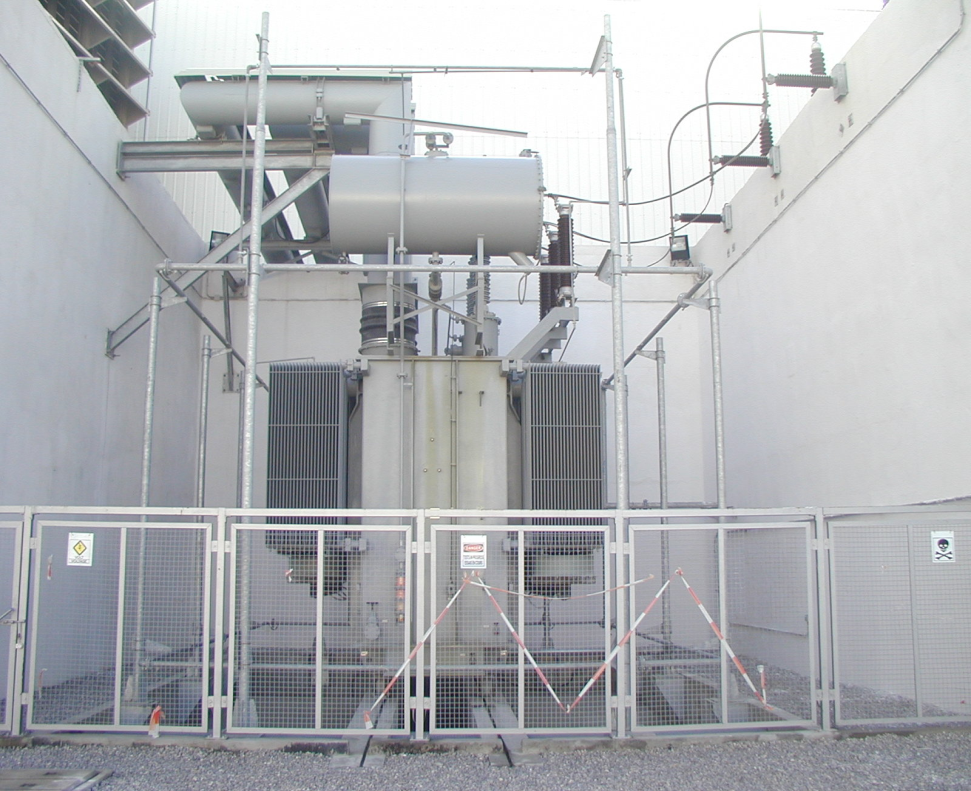
\includegraphics[scale=0.7]{./Figures/tranfo_principal.png}
		\label{fig:trans_princip}

}
\subfigure[Transformateur De Soutirage]{
	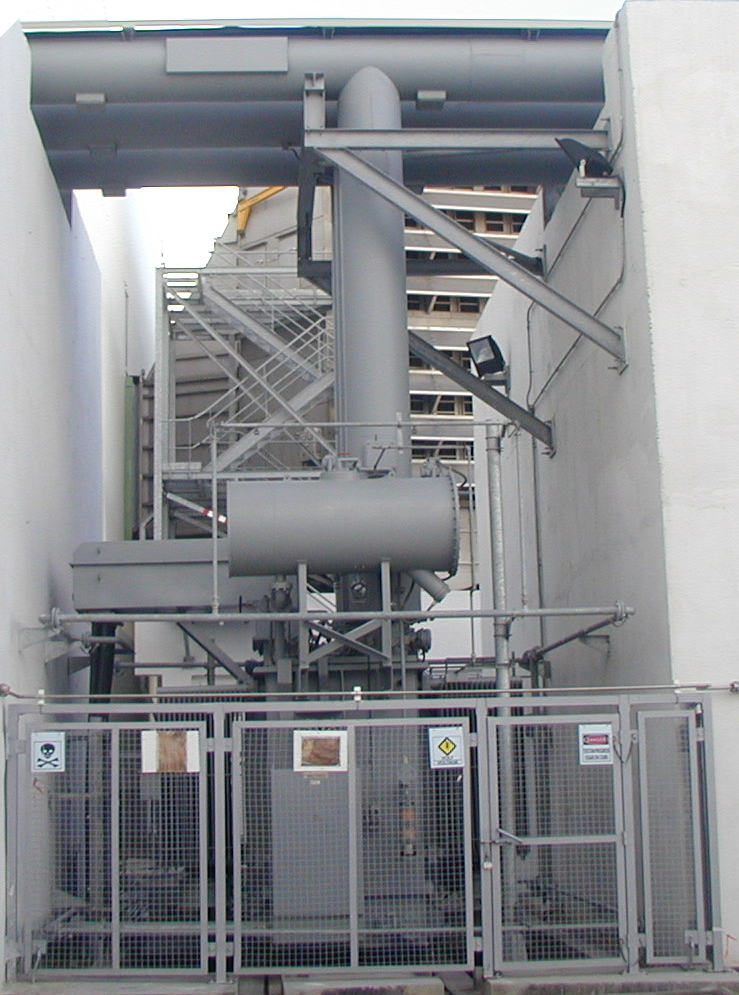
\includegraphics[scale=0.7]{./Figures/tranfo_soutirage.png}

	\label{fig:trans_soutir}
}
\caption{Transformateurs de la centrale}
\label{fig:transformateurs}
\end{figure}



\subsection{Poste de Traitement des eaux}
Cette station satisfait les besoins de la centrale en terme de qualité et type d'eau. A la sortie de ce poste, l'eau est utilisée pour l'alimentation des chaudières, le circuit de refroidissement et d'autres utilisations dans la centrale.
Pour plus de détails sur les différents types d'eaux utilisées dans la centrale, se référer au \hbox{tableau \ref{tab:type_eau} page \pageref{tab:type_eau}}.

\begin{table}[h]
\centering
\begin{tabular}{|c|c|}
\hline
SEI  & (20 \conduct) Eau de service et incendie\\
\hline
SER & (0.06 \conduct) Eau déminéralisé\\
\hline
SRI & (SER + Inhibiteur de corrosion) Eau de réfrigération \\
\hline
CRF & Eau de refroidissement du condenseur \\
\hline
SRA & Eau de refroidissement  du SRI\\
\hline
SEP & Eau de Sonède\\
\hline
\end{tabular}
\caption{Différents eaux de le centrale}
\label{tab:type_eau}

\end{table}

L'eau provenant de la mer entre dans la station avec une conductivité de 55000 \conduct. Elle  en ressort avec  0.06 \conduct. Pour ce faire, la station utilise les équipements suivants :

\begin{itemize}
\item Un pré-filtre
\item	Deux filtres primaires
\item	Deux filtres secondaires
\item Deux filtres à cartouche
\item Un osmoseur  primaire
\item	Un dégazeur
\item Un osmoseur secondaire 
\item	Un système d'électro-ionisation (EDI)
\end{itemize}	
%L'eau de mer sera traitée après avoir passé de différentes étapes.
\begin{figure}

  \begin{minipage}[t]{7cm}
        \centering
	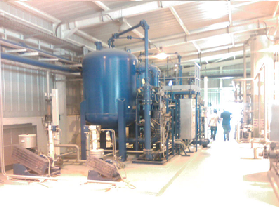
\includegraphics[scale=0.9]{./Figures/filtre.png}
		\label{fig:filtre}
		\caption{Filtre}
    \end{minipage}
    \begin{minipage}[t]{8cm}
        \centering
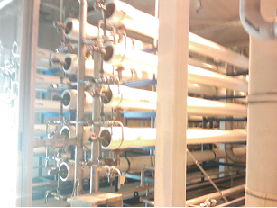
\includegraphics[scale=0.9]{./Figures/osmoseur.png}

	\label{fig:osmoseur}
			\caption{Osmoseur}

    \end{minipage}
\end{figure}

\begin{comment}
Tout d'abord, l'eau passe par un pré-filtre. Ce dernier se charge d'éliminer les corps de taille (exemple algues). L'eau, continue ensuite son chemin à travers un filtre primaire, secondaire et un micro-filtre et pour finir un filtre à cartouche. 
Ceci étant dans le but d'éliminer les matières en suspension avant d'enter dans l'osmoseur.


 \begin{figure}[hbtp]
 \centering
 \includegraphics[scale=2,trim=0cm 4cm 0cm 0 cm,clip=true]{filtration.png}
 \caption{Schéma de filtration}
 \end{figure}
 
Dans l'osmoseur, l'eau passe par 9 tubes contenant chacun 7 membranes et subit le phénomène d'osmose inverse. A sa sortie, on obtient de l'eau douce à 1000 \conduct.

Cette dernière continue à être purifié en passant par le dégazeur dans lequel on élimine les gaz (principalement le CO2).
  
\begin{figure}[t]
\centering
\includegraphics[scale=0.7]{osmose.png}
\caption{Phénomène d'osmose}
\end{figure}

Le processus d'osmose inverse reprend dans l'osmoseur secondaire. Ce dernier est constitué de deux étages contenant deux et un osmoseur respectivement.

L'eau résultante est l'eau de service SEI.

\newpage
Le traitement d'eau ne s'arrête pas à cette étape. Les besoins de la centrale\footnote{L'eau destinée au condenseur et la chaudière doit être très pure afin éviter tout risque de corrosion} l'obligent à considérer un autre traitement : L' électrodéionisation (EDI).

Cette technique est pratiquement l'inverse de l'osmose inverse : \\Des électrodes attirent les ions à travers des membranes. Comme les ions forts sont éliminés du procédé, la conductivité devient alors assez faible.
On obtient à la sortie une eau de conductivité 0.06 \conduct.
\begin{figure}[hbtp]
\centering
\includegraphics[scale=1]{deionisiation.jpg}
\caption{Système d'électrodéionisation}
\end{figure}
\newpage
\end{comment}
\subsection{Station de pompage}
\begin{figure}[h]
\centering
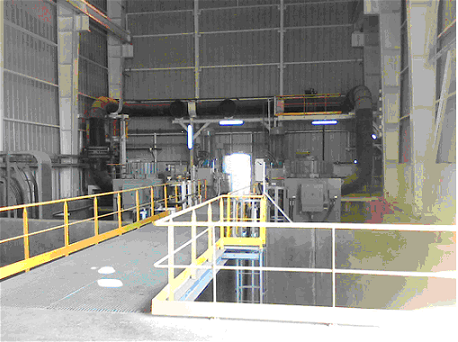
\includegraphics[scale=0.7]{./Figures/stationpompage.png}
\caption{Station de pompage}
\end{figure}
Cette station est placée à l'entrée de la centrale, lieu de proximité de l'eau de mer.


Elle est constituée de : 

\begin{itemize}
\item Trois bassins
\item Deux dégrilleurs 
\item Quatre transmetteur à radar
\item Deux pompes (SRF)
\item Deux  pompes (CRF)

\end{itemize}

\textbf{Bassin principale : }Dans lequel se fait parfois des injections de javel pour se débarrasser des parasites.

\textbf{Bassins secondaires : }Sont deux bassin reliés au bassin principal par deux conduites chacune contenant une grille fine suivie par une grille avancée et un dégrilleur.

\textbf{Dégrilleur : } C'est un dispositif qui sert à nettoyer  manuellement les filtres situés à l'entrée de la station.                                                                                                          

\textbf{Deux  pompes (SRA) : }Servent à envoyer l'eau de mer vers les échangeurs.

\textbf{Deux pompes(CRF) : }Servent à envoyer l'eau de mer vers le condenseur.
\begin{figure}[hbtp]
\centering
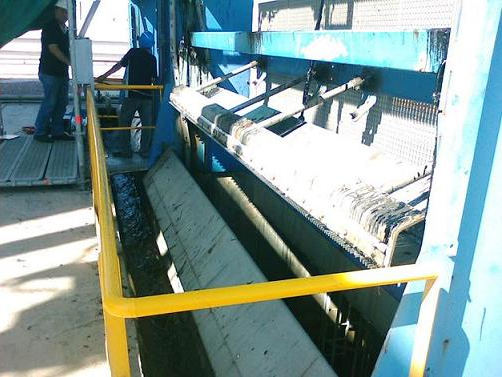
\includegraphics[scale=0.7]{./Figures/degrilleur.png}
\caption{Dégrilleur}
\end{figure}
\begin{figure}[ht]
\centering
\subfigure[Pompe CRF]{
	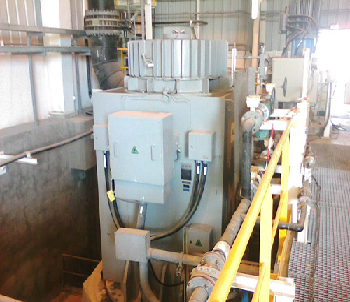
\includegraphics[scale=0.7]{./Figures/CRF.png}
		\label{fig:pompe_crf}

}
\subfigure[Pompe SRA]{
	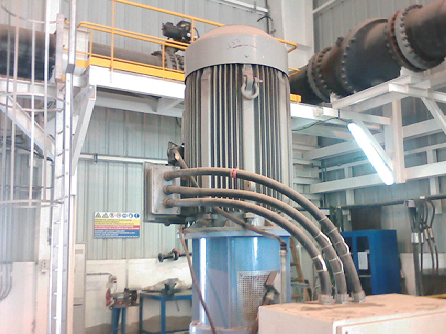
\includegraphics[scale=0.6]{./Figures/SRA.png}

	\label{fig:pompe_sra}
}
\caption{Pompes CRF - SRA}
\label{fig:pompes}
\end{figure}
